\section{Interfejs MPI}

\subsection{Model sieciowy}

Komunikacja odbywa sie za pomocą przesyłania wiadomości (czyli między innymi w standardzie MPI)w tak zwanym modelu sieciowym. Składa się on z określonej liczby procesorów, przy czym każdy z nich posiada własną pamięć lokalną. Procesory posiadają dostęp jedynie do instrukcji i danych przechowywanych w swojej pamięci lokalnej -- nie istnieje pamięć wspólna. Aby umożliwić wymianę informacji pomiędzy procesorami, tworzona jest sieć połączeń (ang \textit{interconnection network}), która zbudowana jest z dwukierunkowych kanałów komunikacyjnych (łącz). 

\begin{figure}[h]
	\centering
	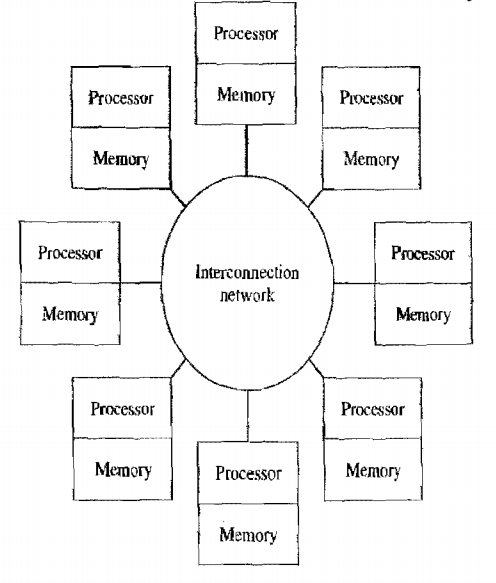
\includegraphics[width=0.85\textwidth]{./img/sieciowy.png}
	\caption{Model sieciowy. Źródło: \cite{Parallel}, str 94}
	\label{img:sieć}
\end{figure}

Wymiana informacji między procesorami jest realizowana poprzez kooperujące ze sobą procedury trasowania (ang. \textit{routing}), które działają w każdym procesorze. Dzięki nim, każdy węzeł sieci (tutaj: procesor) posiada informację, z którymi węzłami może wymieniać informacje. Zbiór wszystkich procedur trasowania definiuje \textbf{topologię sieci połączeń}. Można ją opisać przy pomocy grafu, gdzie wierzchołkami (węzłami) są procedory, natomiast krawędzi to dwukierunkowe łącza.

Ocenę skuteczność/przydatność danej sieci podczas prowadzenia obliczeń równoległych można określić biorąc pod uwagę kilka parametrów:

\begin{itemize}
	\item \textbf{Średnica sieci} (ang \textit{diameter}) -- maksymalna odległość zmierzoną za pomocą liczby krawędzi między dowolnymi dwoma wierzchołkami. Im mniejsza średnica, tym lepsza jest sieć -- oznacza to, że informacje będą potrzebowały średnio mniej czasu na dotarcie do właściwego odbiorcy. Przypadek pesymistyczny zakłada, że wiadomość będzie musiała zostać przesłana przez liczbę krawędzi równej średnicy.
	\item \textbf{Szerokość połowienia sieci} (ang. \textit{bisection width}) -- minimalna liczba krawędzi, którą należy usunąć z obecnej sieci, aby móc ją podzielić na 2 równe podsieci.
	\item \textbf{Szerokość pasma} (ang. \textit{bisection bandwidth}) -- jest to iloczyn szerokości połowienia oraz szybkości przesyłu danych w pojedynczym kanale. Pozwala określić liczbę bitów, jaką można przesłać między połówkami w jednostce czasu. Im większa szerokość pasma, tym lepiej.
	\item \textbf{Maksymalny stopień wierzchołka} -- maksymalna liczba krawędzi połączonych z danym wierzchołkiem (liczona globalnie dla całej sieci). Dla niewielkiego stopnia łatwiej zaprogramować procedury komunikacyjne ze względu na fakt, że używają one mniejszej liczby kanałów. Zakłada się, że sieć jest dobra jeżeli przy wzroście liczby p procesorów średnica sieci rośnie nie szybciej niż logarytmicznie w funkcji p, natomiast maksymalny stopień wierzchołka jest stałą liczbą o małej wartości.
	\item \textbf{Spójność krawędziowa} (ang. \textit{edge connectivity}) -- definiowana jaka minimalna liczba krawędzi, które muszą zostać wyłączone z sieci aby ta stała się niespójna (graf rozłoży się na 2 lub więcej osobnych podgrafów). Im większa spójność krawędziowa, tym odporniejsza jest sieć -- istnieje mniejsze prawdopodobieństwo całkowitego unieruchomienia sieci w przypadku, gdy któryś procesor ulegnie uszkodzeniu. Większa spójność prowadzi też do zmniejszenia rywalizacji poszczególnych węzłów o łącze.
	\item \textbf{Koszt sieci} -- zazwyczaj określana jako suma wszystkich kanałów w sieci.
\end{itemize}

Przykładowe topologie sieci połączeń:

\begin{itemize}
	\item siatka
	\item torus (jedno-, wielowymiarowy)
	\item kostka (jedno-, wielowymiarowa)
\end{itemize}

\begin{figure}[h]
	\centering
	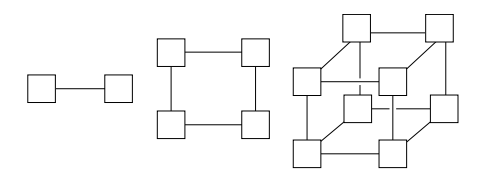
\includegraphics[width=0.85\textwidth]{./img/kostki.png}
	\caption{Topologia kostki. Od lewej: jedno-, dwu- oraz trójwymiarowa. Źródło: \cite{Pacheco}, str 40}
	\label{img:sieć}
\end{figure}

\section{Komunikacja między procesami w biliotece MPI}

\section{Redukcja danych w bibliotece MPI}